% REMEMBER: You must not plagiarise anything in your report. Be extremely careful.

\documentclass{l4proj}

    
%
% put any additional packages here
%

\begin{document}

%==============================================================================
%% METADATA
\title{Accelerating Spaceship Search Using Deep Learning in John Conway's Game of Life}
\author{Paul Bekaert}
\date{September 14, 2018}

\maketitle

%==============================================================================
%% ABSTRACT
\begin{abstract}
    Every abstract follows a similar pattern. Motivate; set aims; describe work; explain results.
    \vskip 0.5em
    ``XYZ is bad. This project investigated ABC to determine if it was better. 
    ABC used XXX and YYY to implement ZZZ. This is particularly interesting as XXX and YYY have
    never been used together. It was found that  
    ABC was 20\% better than XYZ, though it caused rabies in half of subjects.''
\end{abstract}

%==============================================================================

% EDUCATION REUSE CONSENT FORM
% If you consent to your project being shown to future students for educational purposes
% then insert your name and the date below to  sign the education use form that appears in the front of the document. 
% You must explicitly give consent if you wish to do so.
% If you sign, your project may be included in the Hall of Fame if it scores particularly highly.
%
% Please note that you are under no obligation to sign 
% this declaration, but doing so would help future students.
%
\def\consentname {Paul Bekaert} % your full name
\def\consentdate {7 October 2022} % the date you agree
%
\educationalconsent


%==============================================================================
\tableofcontents

%==============================================================================
%% Notes on formatting
%==============================================================================
% The first page, abstract and table of contents are numbered using Roman numerals and are not
% included in the page count. 
%
% From now on pages are numbered
% using Arabic numerals. Therefore, immediately after the first call to \chapter we need the call
% \pagenumbering{arabic} and this should be called once only in the document. 
%
% Do not alter the bibliography style.
%
% The first Chapter should then be on page 1. You are allowed 40 pages for a 40 credit project and 30 pages for a 
% 20 credit report. This includes everything numbered in Arabic numerals (excluding front matter) up
% to but excluding the appendices and bibliography.
%
% You must not alter text size (it is currently 10pt) or alter margins or spacing.
%
%
%==================================================================================================================================
%
% IMPORTANT
% The chapter headings here are **suggestions**. You don't have to follow this model if
% it doesn't fit your project. Every project should have an introduction and conclusion,
% however. 
%
%==================================================================================================================================
\chapter{Introduction}

% reset page numbering. Don't remove this!
\pagenumbering{arabic} 

\section{Motivation}

The game of life has often been seen as a toy project. It is idealistic in its representation, as it is fully observable, episodic and deterministic. However, its simple rules give rise to complex structures that are not easy to find. Those structures can be large, and looking for them is unfeasible with the current methods. In general, conventional graph search methods adapted to the task are are used, but they are slow and require large amounts of memory \cite{list_of_search_algorithms}, and as mentioned, they cannot find objects that are too large. There is, as of yet, no efficient way to search for these structures, and the question remains if there is a way to do it.

The concept of using deep learning to find structures in cellular automata has not yet been explored. With the advent and rise of neural networks, previously thought to be impossible problems have been unlocked, either by solving them directly or speeding up existing search algorithms. Since this is a difficult search problem, it stands to reason that solving it will potentially give new insights into how to solve similar problems.

\section{Aims}

In this paper, we will be trying to find interesting structures in the game of life. Our particular interest will be in oscillating objects that move a set amount of space, so-called 'Spaceships'. The main goal will be to test and see if neural networks can speed up the search, and how different deep learning techniques fare against each other and other conventional search methods. The expectation is that the network will greatly decrease the time it takes to find novel structures or structures already classified as spaceships.

% CHECK THIS 30 VALUE
This search algorithm is especially challenging to implement due to the NP-hardness of the problem. There are $2^{w * h}$ possible structures in a given grid of width and height $w$ and $h$ respectively, from which only $\sim{30}$ structures we're interested in exist. It also bases the functionality of the algorithm on a single hypothesis that is tested in this paper. 

%==================================================================================================================================

\chapter{Background}

\section{The game of life}
% ========

\subsection{Rules}

"The Game of Life" is a zero-player game (a simulation of sorts) invented by John Conway in 1970 which describes a cellular automata (CA) with a set of rules. A cellular automata a simulation of cells evolving every time step, which are represented in a matrix of size $n\times m$. Every time step, the cells are modified using a set of pre-defined rules. In John Conway's Game of life (GoL), a cell is either dead or alive, represented as a $1$ or a $0$ respectively. The neighbourhood of the cell is defined as Moore's neighbourhood, which is the 8 cells adjacent to the cell, diagonally and orthogonally. It can also be thought of as a $3\times 3$ matrix where the subject cell is placed in the middle. The number of neighbours the cell has is the number of cells alive that are present in the cell's Moore neighbourhood, $n$. We can then define the rules of the CA described in Life:

\begin{itemize}
    \item A dead cell turns into a living cell if $n \geq 3$
    \item A dead cell stays dead if $n < 3$
    \item A living cell stays alive if $n = 2$ or $n = 3$
    \item A living cell dies if $n < 2$, due to under-population
    \item A living cell dies if $n > 3$, due to overcrowding
\end{itemize}

A state at $t+1$ is entirely dependant on the current state at $t$ and is calculated using the rules above. The game can go on indefinitely, but usually reaches a state in which cell structure does not change in any significant way. For example, all the cells could die, creating an empty board. More likely however, is that the resulting state will be populated with still-lifes, oscillators, and sometimes spaceships, which are defined below.

\begin{figure}[h]
\centering
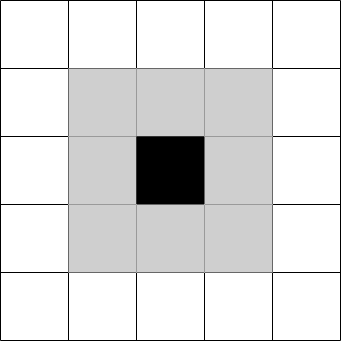
\includegraphics[width=0.4\linewidth]{dissertation/images/diagrams/moores_neighbourhood.png}
\caption{Moore's Neighbourhood}
\label{fig:subim1}

\end{figure}

\subsection{Still lifes}

A still life is a structure that does not move or change shape from generation to generation. They remain static (do not move around the board or in shape), unless outside cells interact with it. Still lifes are by far the most common structures in the GoL, and they are easy to find, as they have the same shape for $t$ and $t+1$. Here are some examples of still lifes:

\begin{figure}[h]
\centering
\begin{subfigure}[b]{0.25\textwidth}
    
\includegraphics[width=\textwidth]{dissertation/images/gol_structures/still_life_1.png} 
    \caption{The Block} %SHOULD I GET RID OF THIS ONE OR RE-DRAW IT SOMEHOW?
    \label{fig:subim1}
\end{subfigure}
\hfill
\begin{subfigure}[b]{0.25\textwidth}
    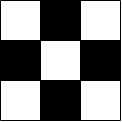
\includegraphics[width=\textwidth]{dissertation/images/gol_structures/still_life_2.png} 
    \caption{The Tub}
    \label{fig:subim1}
\end{subfigure}
\hfill
\begin{subfigure}[b]{0.25\textwidth}
    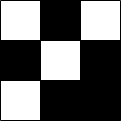
\includegraphics[width=\textwidth]{dissertation/images/gol_structures/still_life_3.png} 
    \caption{The Boat}
    \label{fig:subim1}
\end{subfigure}

\caption{Examples of still lifes}
\end{figure}

\subsection{Oscillators}

These are structures that change shape, but return to the same state every $p$ generations. They are a little harder to detect, as it is impossible to know how many generations it will take for the structure to repeat. An oscillator will stay in the same position after it has oscillated, and will keep oscillating as long as it is undisturbed by other cells and the program keeps running. Here are some examples of oscillators:

\begin{figure}[h]
\centering
\begin{subfigure}[b]{0.4\textwidth}
    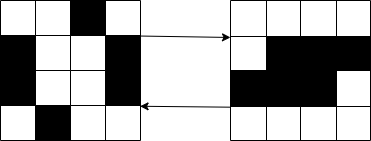
\includegraphics[width=\textwidth]{dissertation/images/gol_structures/toad_transition.png} 
    \caption{The Toad}
    \label{fig:subim1}
\end{subfigure}
\hfill
\begin{subfigure}[b]{0.4\textwidth}
    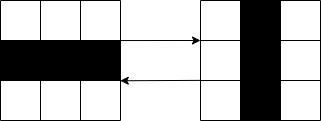
\includegraphics[width=\textwidth]{dissertation/images/gol_structures/blinker_transition.png} 
    \caption{The Blinker}
    \label{fig:subim1}
\end{subfigure}

\caption{Examples of oscillators and their different iterations}
\end{figure}

\subsection{Spaceships}

% TALK MORE ABOUT THEM
Spaceships are the main focus of this paper, and are the hardest structures to detect. They are similar to oscillators in that they repeat their state every $p$ generations. However, they also move a certain distance since their last oscillation. If the state space they are in is unbounded, then they will move forever without changing direction.

The speed of a spaceship is determined in terms of the speed of light of GoL, $c$. This $c$ is defined as 1 cell per second, as it is theoretically the quickest information could hope to propagate given the rules of Life. The ship can move diagonally, orthogonally, or knightwise, which is when a ship moves in an oblique direction. A spaceship with a period $p$, which is moving $n$ cells in a particular direction is said to have a speed $nc/p$. A ship moving $n = 2$ cells left and with a period $p = 5$ will have a speed of $2c/5$. For a ship moving knightwise $n$ cells either left or right, and $m$ cells either up or down, will have a speed denoted as $(m, n)c/p$. These speeds can be simplified, for example a spaceship moving at speed $2c/4$ can be written as $c/2$.

A further way to classify spaceships is by their type. 
% should you explain this?

\begin{figure}[h]
\centering
\begin{subfigure}[b]{0.4\textwidth}
    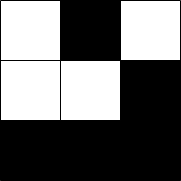
\includegraphics[width=\textwidth]{dissertation/images/gol_structures/glider.png} 
    \caption{The glider}
    \label{fig:subim1}
\end{subfigure}
\hfill
\begin{subfigure}[b]{0.4\textwidth}
    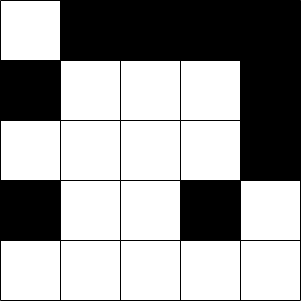
\includegraphics[width=\textwidth]{dissertation/images/gol_structures/LWSS.png} 
    \caption{The LWSS}
    \label{fig:subim1}
\end{subfigure}

\caption{Examples of spaceships}
\end{figure}

Spaceships can be made up of different GoL parts. An oscillator can be joined with another spaceship part to create new spaceships. In addition to this, engineered spaceships can be made arbitrarily large. There are many different type of ships, but only a handful are original ships. Elementary spaceships are the rarest kind of ships: those are the ones which can occur naturally in the GoL, and are relatively small in size.

% ========

\section{Different ways to find spaceships}

The problem we're trying to solve is to find elementary spaceships. These are, as explained above, structures that repeat inside of a game of life grid, but also move a certain amount of space. This is a widely known toy problem, however it is an NP-hard problem, which means brute force is out of the question. In a given $n \times m$ grid, there are $2^{n \times m}$ possible combinations. For example, a glider, which takes at least a $3x3$ grid to be represented, would be found by searching $2^{9}$ grids. Brute force becomes unfeasible after approximately $n > 6, m > 6$. This algorithm tends not to have much use, but it has found a comprehensive list of all still-lives, oscillators, and spaceships within a small rectangle.

A better approach is representing the board as a graph. By representing each cell as a path- a path where the cell is either alive or a path where the cell is dead- a tree search method can be used. This is the method used in most algorithms today, by trying to optimize which cell should be placed next. Some combinations of cells should not be placed together as the result would be incompatible with a spaceship, and therefore the algorithm can eliminate entire sub-trees from the search space.

\section{Existing Search Methods}

There are not many research papers on the subjects, but in Searching for Spaceships \cite{searching_for_spaceships}, a de Bruijn graph is used to represent the cells. The algorithm - "gfind" - only works on one side of the ship, and assumes the other to be symmetrical. A ship is then constructed by applying the GoL rules to rows of the ship, and placing the formed cell in front of the ship in the direction it will move. To visualize this, imagine the grid follows the ship as it is moving, so that the ship looks like it is simply oscillating. A future oscillation can therefore be predicted by taking the evolution of the spaceship for every row of 3, and applying it $p$ (the speed of the ship) cells above the evolution, as it would reach that point p next iteration. This approach has one major drawback- any spaceship that is not a "long" spaceship will not be detected. The search space also does not include non-symmetrical spaceships, of which there are many.

Another well known algorithm to find spaceships or oscillators is "lifesrc" created by David Bell, uses a depth first backtracking search. The grid is first set up with a few 'known' cells, set by the user. The rest of the cells are classed as 'unknown'. When the algorithm starts running, a decision is made on whether a cell should be alive or not, and the program will check forward and backward if there are any oscillating patterns of period $p$ set by the user. If nothing is found, the search continues, using the decided cell. If it is found later on that a cell placement in a particular cell is impossible, or that there are no oscillators in a particular configuration, then the algorithm will backtrack to the latest cell it decided on randomly. This is essentially a depth first search, however it discards certain sub-trees by eliminating ones that do not follow the Life rules (for example, checking if every cell is alive in a $4 \times 4$ grid would be redundant, since almost all cells in that grid would die in the next iteration). 

The most efficient algorithm used to find spaceships today is dubbed the 'ikpx2' algorithm, which was created by Adam P. Goucher. It was inspired by gfind, which searches De Bruijn graphs representing the different parts of a spaceship. However, ikpx reduces the spaceship search problem into a set of SAT constraints, which can then be used on an SAT solver. The solver used in question is the "iglucose" \cite{sat_2018} SAT solver and sped up the search considerably, as a lot of research has gone into accelerating SAT solvers. A notable find by the ikpx2 algorith was the 'knightship': the first oblique spaceship found, or in other words, a spaceships that does not move diagonally nor orthogonally.

\section{Deep Learning with the GoL in General}

There are a few research papers written on neural networks and the game of life, with one notable one being about forward planning in the GoL \cite{game_of_life_dl_is_hard}. In this paper, they    try to predict the future structure of a starting configuration. They used several 1x1 and 3x3 convolutional layers in their network, activated by ReLU functions. Although the model was able to perfectly predict the next iteration of the game, the further the model tries to predict, the worse the result. The problem hypothesised by Springer is the 'lottery ticket problem', in which the starting configuration of the model is what would allow it to converge to a correct solution. [MAKE SURE THIS IS CORRECT AND REPHRASE]

Apart from research done, there are many hobbyists working on combining deep learning with GoL. One of them is James McGuigan, who trained a neural network to learn the game of life after one iteration. He has also worked on reversing the game of life, trying to find a previous configuration using a current board state. Another notable use of deep learning and the game of life is by NeatAI, who used genetic algorithms in the game of life \cite{neatai_gol}. He used a $c$ function that calculates the overall 'complexity' of the current structures in the grid. For example, a grid with random cells is not very interesting, but one that has a couple of gliders and oscillators with high periods may be of more interest. To design his $c£$ function, he took inspiration from a paper by \cite{algorithmic_specified_complexity}, which describes a process of encoding interesting objects in the game of life. It uses features of an object such as shift, repeating period, intersection between 2 or more objects, to define the properties of such an object, These properties are then bit-encoded to form a number that specifies the complexity of the object. To find the complexity of a particular state on a board, the sum of the object complexities is taken.

NeatAI took this $c$ function and applied it to a neural network which determined whether or not a cell should be alive given the input parameters $x$, $y$, population density, and bias. He then used genetic neural networks to improve his model to maximize the $c$ function. The net improved by making optimal start configurations for the model to evolve into. This is an interesting concept, as if the $c$ function were to be changed to be maximised by how far a pattern has reached from the origin, it could potentially be used to find new spaceships for example.


%==================================================================================================================================

\chapter{Analysis}

\section{The Main Assumption}
Neural networks are good at detecting general patterns which can be hard to detect as humans. There has been a lot of debate in the GoL community about an underlying pattern to spaceships. There have been methods by the community which use "spaceship engineering" - combining multiple identified sub-parts of spaceships to make a new moving ship. However, there has yet to be a formalized equation or pattern found to help fast-track the search of such ships. To use a neural network for this problem, the approach taken in this paper revolves around the assumption that spaceships have an underlying pattern which is detectable to a neural network. Although there are not many spaceships, data expansion methods are used to gather more data, and convolutional techniques are used to train the network.

This assumption is also used in the scoring network, as only ships that have been trained on will have a high score, implying that there is also some type of general pattern.

%==================================================================================================================================
\chapter{Design}

\section{The Search Algorithm}

The algorithm is a standard tree search, but uses two neural networks to help accelerate it. The first network is trained to predict the probability change that a cell should be present given a structure. This will then be used in a tree search algorithm, with branches generated given the highest changes in probability. The second network is trained to predict the mean square error of a given configuration. This is to be used as a heuristic for the A* algorithm.

The probability prediction network receives as input a grid of arbitrary size with probability values between 0 and 1. The network will then predict a change in probability grid. The highest changes in probability (positive or negative) are then applied to a new grid. these grids then become the branches of a node. Using the scoring network, the grid with the lowest score is then chosen to be the next node. This is effectively an A* search technique.

\section{The Networks}

There are two main networks that this algorithm will use to guide the search:

\begin{itemize}
    \item The probability network: used to find which cells should be modified
    \item The scoring network: used as a heuristic function
\end{itemize}

The probability network uses a fully convolutional network without pooling layers. Swish activation functions are used between each convolution, and will output a convolution that retains the size of the input. Input of the network consists of a configuration of cells with values ranging from 0 to 1, each representing a probability of a cell being present. The output is then given as a change of probability of the input.

The scoring network also uses a series of convolutions, but is then followed by an average pooling layer, and finally a fully connected layer to predict a final score between 0 and 1. Scoring of this network is used as a heuristic to find how far a given solution is from converging towards a spaceship; the idea being that this problem can be turned into an A* type of search.

% SHOULD THIS BE ANOTHER SECTION INSIDE THE IMPLEMENTATION, TALKING ABOUT HOW THESE MOCK SPACESHIPS WERE CREATED?
\section{Data used to train the network}

In this paper, the search is focused on elementary-like spaceships. Those are spaceships which are quite small (less than $100 \times 100$ in size), that have different speeds, and are usually elementary spaceships but there are a few engineered ships. These ships are classified as "interesting" by the community, and are stored in a database called "new-gliders.db" [CITE HERE]. The resulting dataset is quite small in size, fielding 31 spaceships in total. This is not ideal, as the number of ships should be as big as possible in order to get an idea of a ship pattern that will work well. To mitigate this lack of data, the ships were rotated to face all 4 directions, giving 124 different structures. Next, the ships were evolved in each direction, and all their period transitions were recorded. This expanded the dataset to around 1000 items.

\begin{figure}[h]
\centering
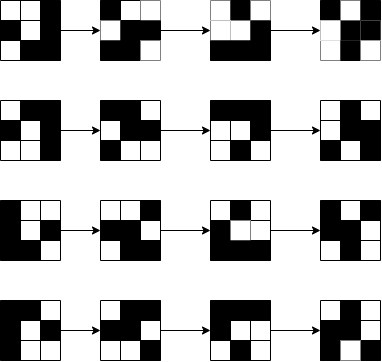
\includegraphics[width=\textwidth]{dissertation/images/diagrams/increasing_ship_data.png} 
\caption{Increasing dataset size by rotating ships in all 4 directions and iterating over all periods. Here you can see the Glider, which went from only 1 item in the dataset to 16.}
\label{fig:subim1}
\end{figure}

The next step of the process is to turn this ship into training data for the network. Several ideas were brainstormed, but the one that made the most sense is as follows: taking an initial spaceship, remove $n$ cells from this ship. At the same time, add a random number of cells sampled from a normal distribution around $n$ in locations where there should be none. Do this for different $n$ values, starting at 1 all the way to the number of cells the ship has. This does several things: it prevents the network from only learning where to place cells; as it also needs to remove them. It also does not let the network count the number of cells as the number of cells is random. This method of deconstruction yields a massive dataset. The final step is to give the network the "change in probability" values. Subtract the actual ship with the deconstructed matrix, and that gives the solution matrix for any given input. This data augmentation method can produce quite a lot of data, with parameters being the ratio of the ship to remove, and the number of cells to add to the structure.
% Maybe mention how this could produce different kind of results and maybe can be optimized to figure out almost completed ships, mid-range, and early range ships?

\begin{figure}[h]
\centering
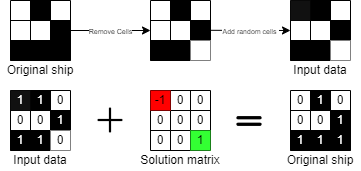
\includegraphics[width=\textwidth]{dissertation/images/diagrams/data_augmentation.png} 
\caption{Creating the input and solution matrices.}
\label{fig:subim1}
\end{figure}

The scoring network used similar data, however it needs to output a score instead of a matrix. The objective of the this network is to model the MSE between a ship and the structure. So, as a solution to a matrix, the MSE error is used as the target for the scoring network. 

%==================================================================================================================================
\chapter{Implementation}

\section{Software Engineering Practices}

Identifying what needed to be done in the project was key to advancing in a timely manner. To do this, I kept an organised file which contained the tasks and objectives of the project, and a set list of things I needed to do within a certain week. In addition to this, I used the waterfall project development method, which suited the project well as it was a clear incremental step-based approach: first design a network to predict good cell probability values, then create a scoring network, and then assemble everything. Each step of the process had to be tested individually and as a whole. I also kept a sheet logging the hours I put in the project, and what I did during those hours. GitHub was used as version control for the project, and to allow my supervisor to access my code easily.

\section {Unsuccessful Attempts}

\subsection{Ship Probability}

My first try to solve this problem revolved over giving structures a "probability" as to how close they are to being a spaceship. The idea was to teach a network the probability of a structure being a ship. A series of convolutions and pooling was used, followed by an adaptive convolutional layer which was then fed to a fully connected network. Given an input, this network would produce a probability of the input being a spaceship. This technique did not work for several reasons: The pooling lost information about the structure, the fully connected network was not able to properly converge, and the output was a softmax which was unreliable as a probability. Furthermore, the training data used on this network was not as complete as the training data used in future trials. Instead of the deconstruction of ships as mentioned in section 4.3, the data it trained on was either a ship or a random collection of cells. There are multiple problem with this, but the main issue would be that a ship would have abundant amounts of dead cells around it, which made them easy to detect by the network. To counter this problem, different density ratios were used, along with reducing the size of the random noise to be that of the size of a spaceship. However, this did little to improve the network, most likely due to its fully connected nature, which failed to converge due to having to learn locality from scratch.

This probability prediction neural network was fed to a tree search which worked by flipping cells off and on and checking if the probability of the structure being a spaceship increased. This did not work very well, partially because the network did not produce good results, but also because the fully connected layer meant that changing a single cell did not change the final output significantly. Large changes in the structure did yield better results, since a greater change in the input would produce a change to the fully connected layer, but was ultimately not useful for finding new ships. 

This initial network may sound familiar: the scoring network used in the search algorithm. However, there is one key difference between the two. While the ship probability algorithm tried to find the \emph{probability} of a structure being a ship, the scoring model tries to model the \emph{positive MSE loss} of a structure to a spaceship. The positive MSE loss is essentially the same as MSE loss: however the higher the value the better the score. This scoring function is more reliable than a probability, as it best represents how 'close' the ship is to being complete, which is what the search algorithm converges towards.

\subsection {Stochastic Ship Cell Probability}

This second method attempted was similar to the method being used now. As mentioned, the value of every cell is represented as the probability of a cell being alive. This originally came from the idea that perhaps a stochastic version of the search algorithm could be used: activate cells based on the probability of them being alive, and then check if it is a spaceship. Repeat this until the probabilities are polarised to one side or the other. This did not work for several reasons: the stochastic nature of this search algorithm did not fit well with an NP-hard problem, which meant poor rate of convergence. In addition to this, the network training did not fit well enough to be used in a probabilistic manner. Since the model was trained on 1s and 0s, applying the network output on itself would give the same exact output from the last iteration, which meant there was no change of input for the model. Furthermore, since there are on average a large amount of dead cells in any given spaceship, the model was trained to decrease probabilities everywhere. This means that after a few iterations, the probability of any cell was 0.
%This could have worked if more data was used, but the dataset used for the current search algorithm was already huge?

\section{Challenges faced}

Finding spaceships has been a challenge many in the GoL community have attempted, mostly using algorithmic methods and logical tree search programs. However, there is close to no research done on deep learning in the game of life, and no one has tried to find spaceships before. This made it very hard to base the program off previous research. 

The network took a huge amount of data. This coupled with the fact that several convolutions are needed, training the network took days. Due to the limited time available, testing new networks was difficult, as training had to take place on another computer with a better GPU. This meant that even small changes to convolution size or other such parameters would take days to get results, and slowed down the testing process significantly.

As mentioned previously in [the data section], there were not many spaceships to work with. Even if there exists a general pattern to spaceships as indicated in [the main assumption chapter], the lack of data may mean that this general pattern is impossible to identify. With more spaceships, a solution might be easier to converge on.

The search problem is NP-hard. Any conventional algorithm would be extremely slow in navigating the search space. The main aim of the paper is to accelerate this search using deep learning, but the problem remains very difficult. Coupled with the fact that no previous work has been done on this subject, 

Another issue was overfitting. It is very hard to get good results, and any that are found are most likely due to the network learning how to overfit the spaceship results. To mitigate this, I trained the network on a subset of the entire dataset.

\section{Probability Search}

\subsection{Choice of Technologies}

This project is the first time I ever used deep learning to complete a project, which meant I needed a quick and easy introduction into deep learning. The most obvious choice as someone who is good with Python and has never done any sort of machine learning was PyTorch. It allows for quick assembly of a neural network in python, and can be easily tested. Numpy was essential to allow rapid evaluation of GoL states. Since the code involves a lot of transformations of matrices, Numpy was perfect for quick and easy computation. Pandas and matplotlib were used heavily for the evaluation of my search method.

PYGAME

\subsection{Architecture of the networks}

The probability network uses a series of convolutions and swish activation functions to find the given change of probability in a cell. The use of the convolutions is to encourage locality. In the GoL, only the cells in Moore's neighbourhood are considered (those directly adjacent). Therefore, it follows that a convolutional network would be the best fit, as the probability of a cell being present on a spaceship would largely depend on cells close to it. However, not only $3 \times 3$ filters were used. Near the end of the network, it was found that using $5 \times 5$ filters were very effective, which could be due to larger cell patterns depending on one another to fully move a ship. In between the $3 \times 3$ and $5 \times 5$ layers, a $1 \times 1$ layer was added. The argument behind this convolution is to modify individual cells which are more or less important based on where they are. This network was trained with the aforementioned "ratio deconstruction" method.

\begin{figure}[h]
\centering
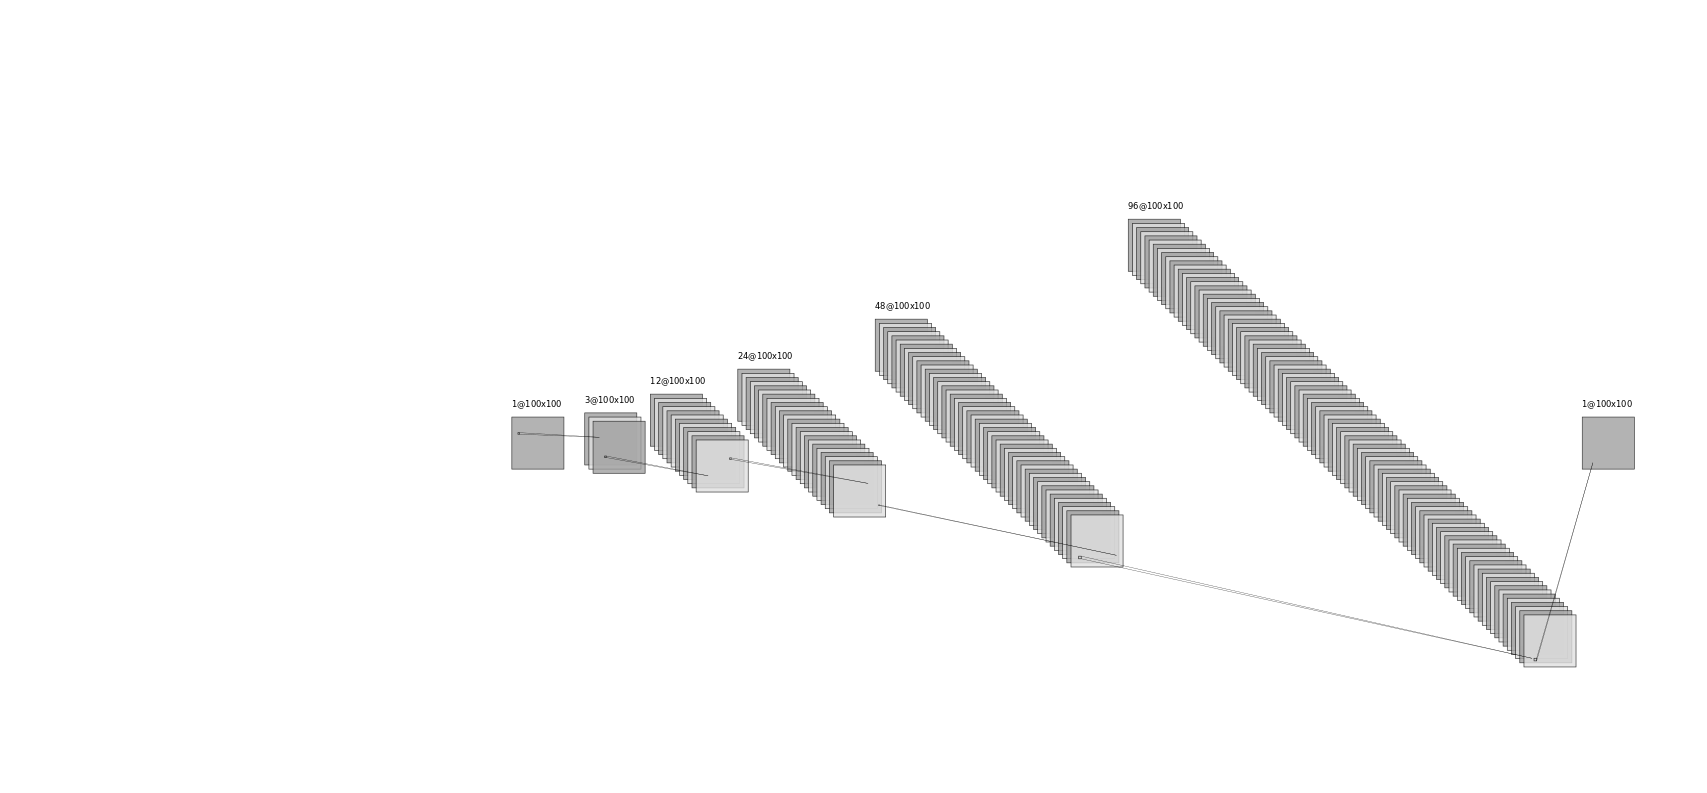
\includegraphics[width=0.8\linewidth]{dissertation/images/diagrams/probability_network_diagram.png}
\caption{Cell Probability change network}
\label{fig:subim1}
\end{figure}
\begin{figure}[h]
\centering
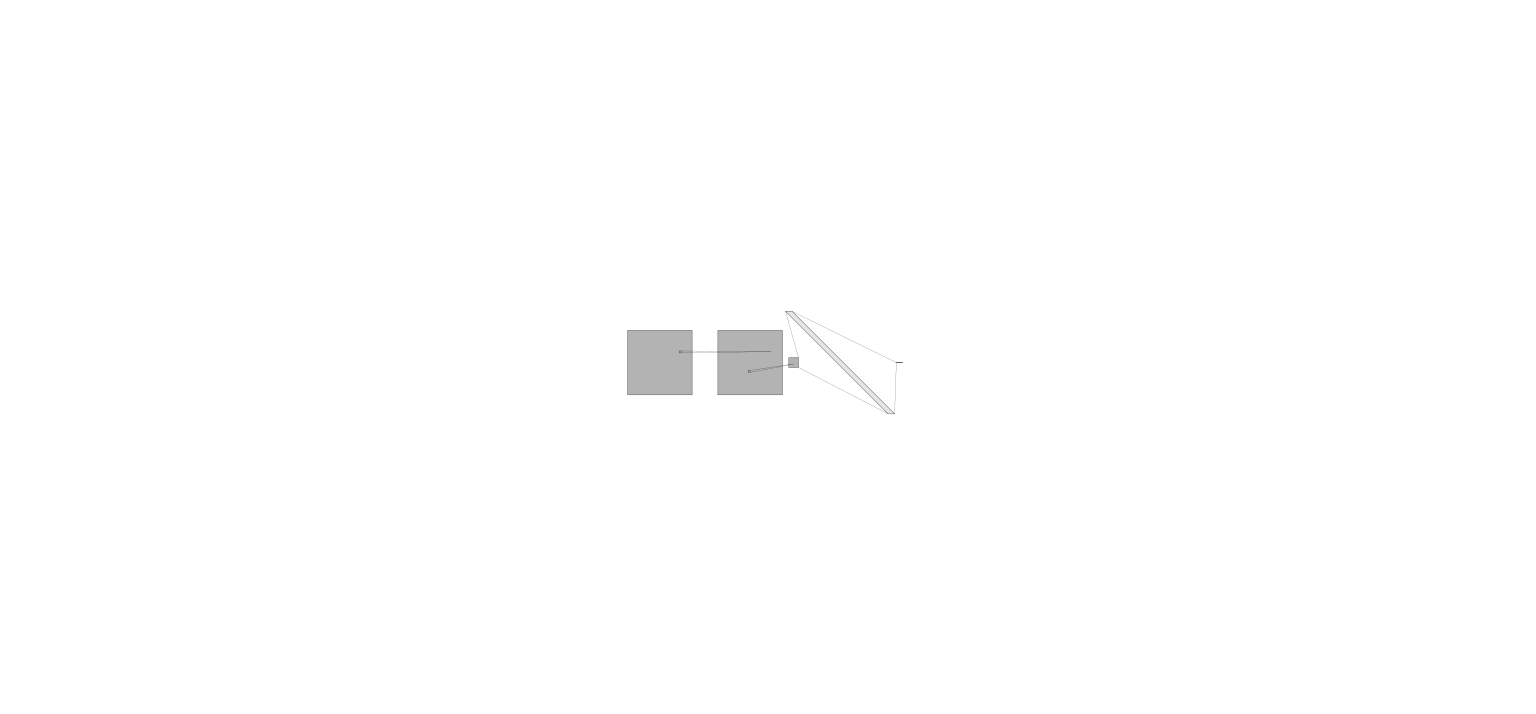
\includegraphics[width=0.8\linewidth]{dissertation/images/diagrams/scoring_network_diagram.png}
\caption{Scoring network architecture}
\label{fig:subim1}
\end{figure}

The scoring network works in a similar manner, with the exception of a average pooling layer before feeding the output into a fully connected network, which then outputs a score. This network also assumes that ships have a general underlying structure that can be detected by the convolutional network, and is different to the original ship probability function as it tries to model an existing function, and not a linear probability function. The goal of the network is to score structures that are close to being a spaceship higher, and to score structures that are further from being a spaceship lower. [EXPLAIN WHY THE MSE LOSS IS SCORED HIGHER WHEN CLOSER TO THE SHIP]

\subsection{Graph search}

The graph search was relatively simple and is based off of A*. The search starts with a few "set" cells which is generated by the algorithm or by the user. This initial grid is fed to the model, which returns a change of probability value for each cell in the grid. The top $n$ cells with the greatest magnitude of are then used to create $n$ alternative board configurations. These are turned into nodes, and are scored using the scoring network, which tries to model an inverse mean squared error of the current grid to a spaceship. This is then used to pick the node with the highest value. Once a node has been chosen, the previous node is added to the list of explored nodes, and has a $n_visited$ attribute which is incremented. If there are no nodes to explore, the search algorithm will use this list to pick the next node. To assure that cells are not being switched randomly, a threshold value is added to prevent candidate cells with very small probability changes. If this value is not achieved, then there are no candidate states selected, which leads the algorithm down the visited path. This is done $max_depth$ times. Once the max depth has been reached, a list of the best nodes found is returned. This is then used by an improvement function, which finds all the cells in common of each node. This is turned into a new initial node for the tree search, and fed back to the algorithm. This is done repeatedly until a number of iterations has expired. Individual ships found are reported at the end, along with their statistics and characteristics.

\subsection{General steps of search}

\begin{figure}[h]
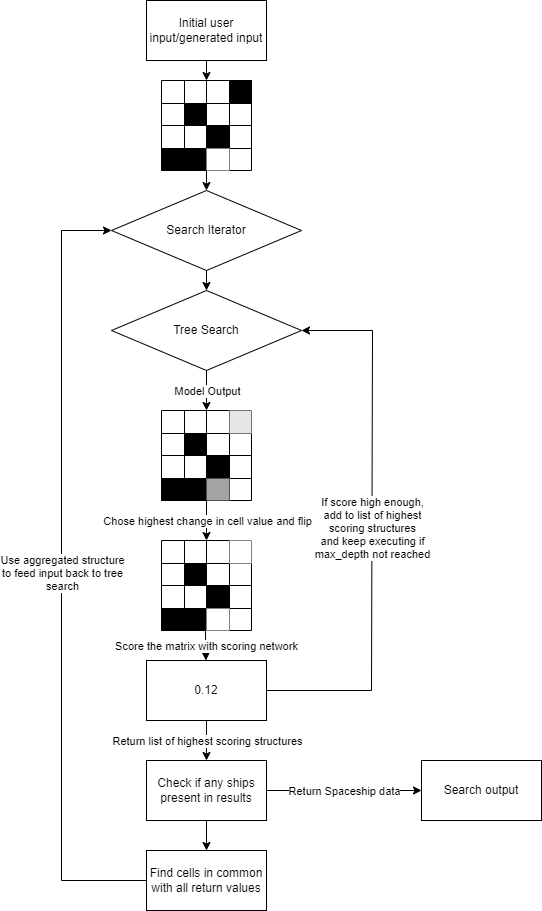
\includegraphics[width=0.9\linewidth, height=20cm]{dissertation/images/diagrams/gol_search_structure.png}
\caption{Search method architecture}
\label{fig:subim1}
\end{figure}

\subsection{Iterating over the tree search}

One main idea of the search is using the outputs of the tree search and returning a new input node which looks at common cells used in the outputs. This does two things: it prevents the tree search from branching too far away from the solution, and it shortens the node list making the search faster. When the tree search gets close to the solution, it has been observed that finding the correct cell which will fix the ship is difficult. This is most likely due to the scoring function: since MSE is a squared error function, the error is exponential in nature. When the algorithm comes close to converging to a solution, the change in score is almost insignificant. This leads the tree search to accidentally change the wrong cell, and therefore get stuck in a loop where it is essentially using trial and error to get the correct cell. By cutting the tree search at an early $max_depth$, the input can be re-organised to (hopefully) only include the core cells important to the ship, and re-input them in the tree search. The second advantage of using this technique is that it prevents the visited list from getting too large. After a certain point, the visited list can get quite large [CHECK THIS] and may lead to the program slowing down. 

One major drawback of using this method is it may cut a solution early. If the tree search is almost at the solution, then re-starting form the core cells may cause issues, as the program may get stuck in a loop of going down the same path, producing the same outputs, and therefore never creating a new output. Also, a ship check is carried out every iteration, which is a costly operation and slows down the algorithm quite a bit.


% PUT THIS IN TOOLS?
\subsection{Determining if a structure is a ship}

This process was used in a relatively straightforward manner. First, a maximum period search time is defined, $p$. This value will be the maximum period a found spaceship can have, which is used to prevent a structure from evolving forever. The idea is to take the structure, place it in an expanded empty grid, and evolve it until it has reached its initial state. The main drawback of this method is that ships which have a period above $p$ will not be detected. Furthermore, this approach is inherently slow: with $p$ iterations and $n$ spaceships needed to be checked, it is quite heavy on the search.

% SHOULD I EVEN INCLUDE THIS
\subsection{Other approaches for choosing next state}

There were 2 other methods thought about for choosing the next state. The first was to re-apply the network output on itself for a set amount of iterations. This, in theory, would create an output that would most resemble a spaceship in terms of what the network thinks will be the spaceship. However, a major problem with this network is that the output is very negative (cell probability changes tend to be negative), which is due to the large amount of dead cells in any given spaceship. If the network output is re-applied to itself several times, information could be lost due to cell probabilities converging towards 0. This is why the branched cell-by-cell approach was selected: the probability does not converge toward 0, and the cell count can increase as well as decrease based on the output of the scoring function.

The second method is the greedy method, where the cell with the greatest change in probability is flipped, and used as input for iteration. This method completely disregards the scoring network and relies solely on the probability network, which could cause erratic behaviour. For example, a loop could be created whereby the greatest change in cell value is a particular cell whether it is on or off, causing the tree search to continually flip the cell, preventing it from converging towards a solution.

% ANALYSIS FUNCTIONS MADE? -> EVALUATION?
% SOME SORT OF TESTING OF THE NETWORKS -> EVALUTATION?

\section{Tools Created and Used}

\subsection{RLE Value Manipulation}

Since storing a GoL matrix is quite expensive, a compression method is used to store structures. It is a type of run length encoding (RLE), which denotes the cells that are alive. It is used a lot when generating training data for the different networks. The token used in this encoding are as follows:

\begin{itemize}
    \item $b$ : dead cell
    \item $o$ : alive cell
    \item $\$$ : end of line
\end{itemize}

The RLE values for spaceships used in the ship search were stored in a text file which needed to be extracted and processed [EXPAND ON THIS]
% TALK ABOUT HOW RLE VALUES HAD TO BE EXTRACTED AND PROCESSED

\subsection{The Game of Life}

To execute some parts of the program, such as the spaceship check method, a GoL implementation was needed. There are some existing tools in python to run the GoL, namely "Golly", which is used in some python search algorithms like "gfind". The use of Golly was considered in the project, however its lack of versatility, poor documentation, and difficulty in adding test code led to the decision of creating an independent GoL tool using numpy. This allowed great leverage of the code, and made different kinds of step-by-step analyses easier to manage. The cells are represented in an $n \times m$ numpy matrix, and every time step a neighbour matrix is applied to find the number of neighbours of an individual cell. With this information, the rules of the GoL can be applied, and a new matrix representing the next time step is produced. 

Inside of this GoL implementation, several sub-tools were produced, such as:
\begin{itemize}
    \item A function to return the next time step, or the state after $t$ time steps 
    \item Representation of the current board using Pygame / matplotlib
    \item Ship data calculator: extracts the speed, size, and general properties of a structure
    \item Structure manipulations: normalizing a structure to fit the RLE encoding, extracting a structure from noise, putting a structure into a sandbox (empty grid) environment
\end{itemize}

These methods were used at various points, from training the networks, to analytics. Further modifications of the GoL code allowed structure data (such as average neighbours, average number of cells over time, changes in cell values) to be extracted, which could not be done with Golly. 

% SHOULD I TALK ABOUT THIS HERE
\subsection{Analytical Tools}


\section{Hyperparameter tuning}

The search algorithm has the following attributes to tune:

\begin{itemize}
    \item $max_depth$ : how deep should the tree go before ending a search iteration
    \item $n_iterations$ : how many tree searches should be done with re-calibrated input
    \item $n_considerations$ : the number of possible cells that the tree search can pick from
    \item Threshold values : the threshold value for a cell to be considered as an addition to the network, % YOU SHOULD PROBABLY DO THIS THE OTHER WAY AROUND TOO, A THRESHOLD FOR REMOVING FROM THE NETWORK?
\end{itemize}

% FOCUS ON WHY ITS IMPORTANT AS WELL AS WHAT HAPPENED
% Parameter tuning was a vital part of making the search process work properly. Initially, the search algorithm worked by flipping cell values that are above 0.5.


%==================================================================================================================================
\chapter{Evaluation} 

\section{Different Testing methods}

\subsection{Probability network}

The probability network has two main functions: to reduce the probability of a cell that is unlikely to be in a spaceship, and to increase the probability of a cell likely to be in a spaceship. This was tested by taking the mean increase in values. For cells that are not part of the spaceship (so called "undesirable cells"), the mean probability increase should be negative. For cells we want in the structure as they are part of a spaceship (desirable cells), the score should be positive. For cells which are not present in the structure and are not desired, the score should be 0. Same for the cells already present in the structure which should stay in the structure: there should be no change in probability. 

The network was scored by taking away a set number of cells, and checking the model output. To test and see what worked best with the model, the model output was fed into the input multiple times. There are 3 scores calculated:

\begin{itemize}
    \item Positive score: the mean value in desirable cells (the higher the better)
    \item Negative score: the mean value in undesirable cells (the lower the better)
    \item Intactness score: the mean value of cells in the structure that need to stay in the structure (the higher the better)
    \item Cohesion score: the mean value of cells added to the structure that need be removed (the lower the better)
\end{itemize}

The best model trained had the following results:

\begin{figure}[h]
\centering
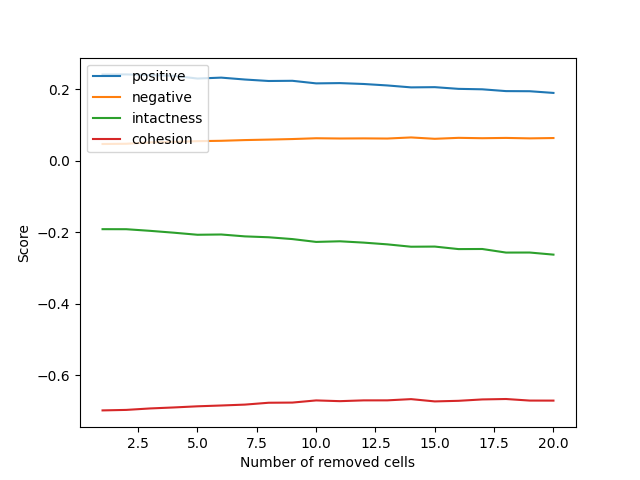
\includegraphics[width=0.6\linewidth]{dissertation/images/graphs/n_removed_cells_score_probability_analysis.png}
\caption{Number of removed cells to score}
\label{fig:subim1}
\end{figure}

As can be seen by the graph, the results are mixed. Although the positive value is high, it is quite close to the negative value. Ideally, the negative line would've been more negative, however it is positive in value, meaning that applying the probability change network on itself would, on average, increase the probability of cells which should not be present. The intactn ess score is also low. In an idea scenario, the intactness score would be at the very least above 0: cells already part of the ship should not be removed. Finally, the cohesion score is quite good: the value is on average very negative, meaning cells which are not supposed to be present are being removed by the model network.

% how should I compare this to see if it is statistically significant? some sort of p-value or something

\subsection{Scoring network}

The scoring network was tested quite easily: it needed to reflect a MSE graph. However, the objective of the network is to increase the score as the MSE decreases. HOW DID I MANAGE TO DO THIS? I HONESTLY DONT KNOW

The MSE was calculated for a different $n$ number of cells removed, and put in a graph.

\subsection{Search}

The outputs of the search could be manipulated in several ways to produce evaluation metrics. 

\begin{itemize}
    \item The number of cells missing: Number of desirable cells not part of the structure
    \item The number of cells extra: Number of undesirable cells
    \item The MSE score from to the target spaceship
    \item The chance of reconstruction given number of cells missing from original ship
\end{itemize}


\section{Results}
`

%==================================================================================================================================
\chapter{Conclusion}    


\section{Guidance}
\begin{itemize}
    \item
        Summarise briefly and fairly.
    \item
        You should be addressing the general problem you introduced in the
        Introduction.        
    \item
        Include summary of concrete results (``the new compiler ran 2x
        faster'')
    \item
        Indicate what future work could be done, but remember: \textbf{you
        won't get credit for things you haven't done}.
\end{itemize}

%==================================================================================================================================
%
% 
%==================================================================================================================================
%  APPENDICES  

\begin{appendices}

\chapter{Appendices}

Typical inclusions in the appendices are:

\begin{itemize}
\item
  Copies of ethics approvals (required if obtained)
\item
  Copies of questionnaires etc. used to gather data from subjects.
\item
  Extensive tables or figures that are too bulky to fit in the main body of
  the report, particularly ones that are repetitive and summarised in the body.

\item Outline of the source code (e.g. directory structure), or other architecture documentation like class diagrams.

\item User manuals, and any guides to starting/running the software.

\end{itemize}

\textbf{Don't include your source code in the appendices}. It will be
submitted separately.

\end{appendices}

%==================================================================================================================================
%   BIBLIOGRAPHY   

% The bibliography style is abbrvnat
% The bibliography always appears last, after the appendices.

\bibliographystyle{abbrvnat}

\bibliography{l4proj}

\end{document}
